\documentclass[11pt,preprint, authoryear]{elsarticle}

\usepackage{lmodern}
%%%% My spacing
\usepackage{setspace}
\setstretch{1.2}
\DeclareMathSizes{12}{14}{10}{10}

% Wrap around which gives all figures included the [H] command, or places it "here". This can be tedious to code in Rmarkdown.
\usepackage{float}
\let\origfigure\figure
\let\endorigfigure\endfigure
\renewenvironment{figure}[1][2] {
    \expandafter\origfigure\expandafter[H]
} {
    \endorigfigure
}

\let\origtable\table
\let\endorigtable\endtable
\renewenvironment{table}[1][2] {
    \expandafter\origtable\expandafter[H]
} {
    \endorigtable
}


\usepackage{ifxetex,ifluatex}
\usepackage{fixltx2e} % provides \textsubscript
\ifnum 0\ifxetex 1\fi\ifluatex 1\fi=0 % if pdftex
  \usepackage[T1]{fontenc}
  \usepackage[utf8]{inputenc}
\else % if luatex or xelatex
  \ifxetex
    \usepackage{mathspec}
    \usepackage{xltxtra,xunicode}
  \else
    \usepackage{fontspec}
  \fi
  \defaultfontfeatures{Mapping=tex-text,Scale=MatchLowercase}
  \newcommand{\euro}{€}
\fi

\usepackage{amssymb, amsmath, amsthm, amsfonts}

\def\bibsection{\section*{References}} %%% Make "References" appear before bibliography


\usepackage[round]{natbib}

\usepackage{longtable}
\usepackage[margin=2.3cm,bottom=2cm,top=2.5cm, includefoot]{geometry}
\usepackage{fancyhdr}
\usepackage[bottom, hang, flushmargin]{footmisc}
\usepackage{graphicx}
\numberwithin{equation}{section}
\numberwithin{figure}{section}
\numberwithin{table}{section}
\setlength{\parindent}{0cm}
\setlength{\parskip}{1.3ex plus 0.5ex minus 0.3ex}
\usepackage{textcomp}
\renewcommand{\headrulewidth}{0pt}

\usepackage{array}
\newcolumntype{x}[1]{>{\centering\arraybackslash\hspace{0pt}}p{#1}}

%%%%  Remove the "preprint submitted to" part. Don't worry about this either, it just looks better without it:
\makeatletter
\def\ps@pprintTitle{%
  \let\@oddhead\@empty
  \let\@evenhead\@empty
  \let\@oddfoot\@empty
  \let\@evenfoot\@oddfoot
}
\makeatother

 \def\tightlist{} % This allows for subbullets!

\usepackage{hyperref}
\hypersetup{breaklinks=true,
            bookmarks=true,
            colorlinks=true,
            citecolor=blue,
            urlcolor=blue,
            linkcolor=blue,
            pdfborder={0 0 0}}


% The following packages allow huxtable to work:
\usepackage{siunitx}
\usepackage{multirow}
\usepackage{hhline}
\usepackage{calc}
\usepackage{tabularx}
\usepackage{booktabs}
\usepackage{caption}


\newenvironment{columns}[1][]{}{}

\newenvironment{column}[1]{\begin{minipage}{#1}\ignorespaces}{%
\end{minipage}
\ifhmode\unskip\fi
\aftergroup\useignorespacesandallpars}

\def\useignorespacesandallpars#1\ignorespaces\fi{%
#1\fi\ignorespacesandallpars}

\makeatletter
\def\ignorespacesandallpars{%
  \@ifnextchar\par
    {\expandafter\ignorespacesandallpars\@gobble}%
    {}%
}
\makeatother

\newenvironment{CSLReferences}[2]{%
}

\urlstyle{same}  % don't use monospace font for urls
\setlength{\parindent}{0pt}
\setlength{\parskip}{6pt plus 2pt minus 1pt}
\setlength{\emergencystretch}{3em}  % prevent overfull lines
\setcounter{secnumdepth}{5}

%%% Use protect on footnotes to avoid problems with footnotes in titles
\let\rmarkdownfootnote\footnote%
\def\footnote{\protect\rmarkdownfootnote}
\IfFileExists{upquote.sty}{\usepackage{upquote}}{}

%%% Include extra packages specified by user

%%% Hard setting column skips for reports - this ensures greater consistency and control over the length settings in the document.
%% page layout
%% paragraphs
\setlength{\baselineskip}{12pt plus 0pt minus 0pt}
\setlength{\parskip}{12pt plus 0pt minus 0pt}
\setlength{\parindent}{0pt plus 0pt minus 0pt}
%% floats
\setlength{\floatsep}{12pt plus 0 pt minus 0pt}
\setlength{\textfloatsep}{20pt plus 0pt minus 0pt}
\setlength{\intextsep}{14pt plus 0pt minus 0pt}
\setlength{\dbltextfloatsep}{20pt plus 0pt minus 0pt}
\setlength{\dblfloatsep}{14pt plus 0pt minus 0pt}
%% maths
\setlength{\abovedisplayskip}{12pt plus 0pt minus 0pt}
\setlength{\belowdisplayskip}{12pt plus 0pt minus 0pt}
%% lists
\setlength{\topsep}{10pt plus 0pt minus 0pt}
\setlength{\partopsep}{3pt plus 0pt minus 0pt}
\setlength{\itemsep}{5pt plus 0pt minus 0pt}
\setlength{\labelsep}{8mm plus 0mm minus 0mm}
\setlength{\parsep}{\the\parskip}
\setlength{\listparindent}{\the\parindent}
%% verbatim
\setlength{\fboxsep}{5pt plus 0pt minus 0pt}



\begin{document}



\begin{frontmatter}  %

\title{Predicting the best 2022/23 fantasy premier league team per game
week}

% Set to FALSE if wanting to remove title (for submission)




\author[Add1]{Austin Byrne}
\ead{22582053@sun.ac.za}





\address[Add1]{Stellenbosch University, South Africa}


\begin{abstract}
\small{
This project aims to predict the best possible fantasy premier league 11
for each game week of the 2022/23 premier league season. The machine
learning model that will be used is a random forests model. To perfect
the model, hyper parameter tuning will be conducted to obatain the
optimal parameter values.
}
\end{abstract}

\vspace{1cm}





\vspace{0.5cm}

\end{frontmatter}

\setcounter{footnote}{0}


\renewcommand{\contentsname}{Table of Contents}
{\tableofcontents}

%________________________
% Header and Footers
%%%%%%%%%%%%%%%%%%%%%%%%%%%%%%%%%
\pagestyle{fancy}
\chead{}
\rhead{}
\lfoot{}
\rfoot{\footnotesize Page \thepage}
\lhead{}
%\rfoot{\footnotesize Page \thepage } % "e.g. Page 2"
\cfoot{}

%\setlength\headheight{30pt}
%%%%%%%%%%%%%%%%%%%%%%%%%%%%%%%%%
%________________________

\headsep 35pt % So that header does not go over title




\hypertarget{introduction}{%
\section{\texorpdfstring{Introduction
\label{Introduction}}{Introduction }}\label{introduction}}

The aim of this project is to create predictions on how many fantasy
premier league points premier league players will score for each game
week. Using these predictions I will be able to select the best fantasy
premier league team which consists of 11 players. The fantasy premier
league team restrictions make this more difficult than just selecting
the top 11 players with the highest predicted points in a game week. The
restrictions consist of only being allowed to have a maximum of 3
players from the same premier league team, your fantasy premier league
team can not have a combined total value that exceeds 100 million and
your team has too stick to certain formations which constrains the
amount of players you can have in each position.

The machine learning model that will be used for these predictions is a
random forests model. The layout of the project consists of data
analysis section. Next, a base line random forests model will be created
and evaluated by calculating the mean absolute error. Next using hyper
parameter tuning the optimal values for the mtry, k-fold and ntree
parameter values will be found. Next a new, tuned random forests model
will be created and it's model performance will also be evaluated via
the mean absolute error. Next, the best model will be used to create
predictions on the amount of points that will be scored by each player
in the 2022/23 premier league season. From these predictions a function
will be created and used that will select the best fantasy premier
league team to select per game week for the 2022/23 premier league
season given the fantasy team restrictions.

\hypertarget{data-exploration}{%
\section{Data exploration}\label{data-exploration}}

The data sets used

The data used for this project are two data sets one for the 2021/22
premier league season and another for the 2022/23 premier league season.
The data used is from the github of vaastav/Fantasy-Premier-League. The
data consists of variables such as the name of each player in the
premier league for that season, which team they play for, which position
they play in, each players individual creativity scores, threat scores,
how many goals they scored, how many goals they conceded, the game week,
value etc.

The 2021/22 data set will be used to train and test the model and the
predictions will be made on the 2022/23 data set.

\hypertarget{correlation-plot-between-player-attributes-and-total-points}{%
\subsection{Correlation plot between player attributes and total
points}\label{correlation-plot-between-player-attributes-and-total-points}}

\begin{figure}[H]

{\centering \includegraphics{Fantasy_premier_league_team_prediction_files/figure-latex/unnamed-chunk-2-1} 

}

\caption{Player attributes correlation plot\label{Figure1}}\label{fig:unnamed-chunk-2}
\end{figure}

The above \ref{Figure1} represents a correlation plot of player
attributes for the 2021/22 premier league season for the purpose of
identifying which player attributes have the biggest impact on total
points earned by players. This is valuable information as we can then
add these most prominent variables into our random forests model as
features in an attempt to obtain accurate prediction results. It is
important to understand that only variables that can be obtained before
a game week must be evaluated.

From \ref{Figure1} it is evident that a players influence score,
ict\_index, threat, selected, transfers in and creativity scores are
positively correlated to the total points variable, which is the
variable we are trying to predict (the target variable). Thus, when
building our random forests model these variables must be added.
Furthermore, we must now look at the correlation between total points
and team attributes.

\hypertarget{correlation-plot-between-team-attributes-and-individual-player-points}{%
\subsection{Correlation plot between team attributes and individual
player
points}\label{correlation-plot-between-team-attributes-and-individual-player-points}}

\begin{figure}[H]

{\centering 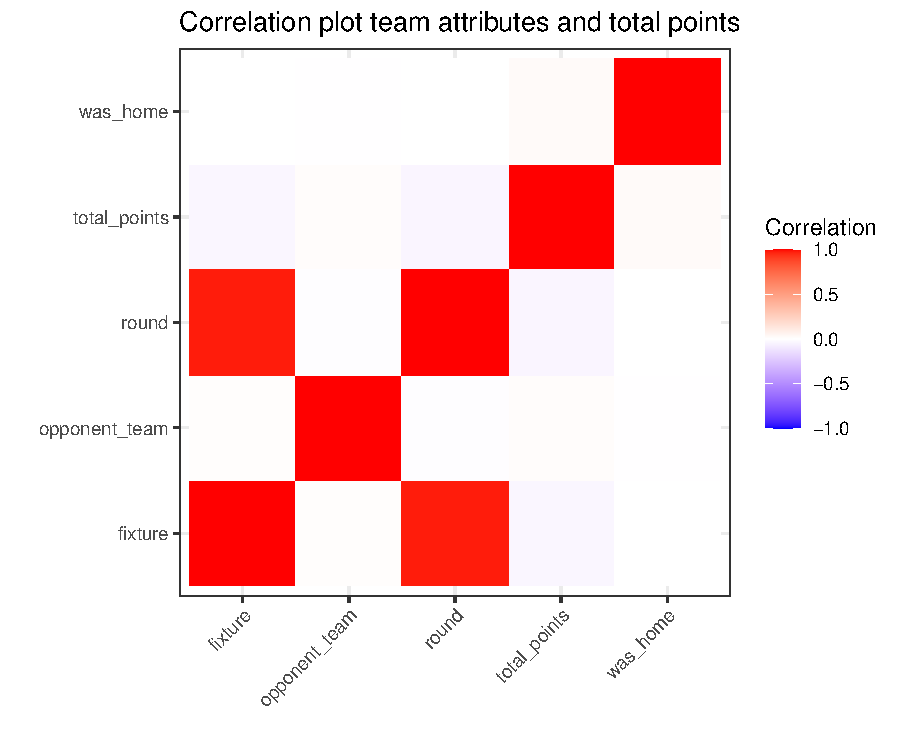
\includegraphics{Fantasy_premier_league_team_prediction_files/figure-latex/unnamed-chunk-3-1} 

}

\caption{Team attributes correlation plot\label{Figure2}}\label{fig:unnamed-chunk-3}
\end{figure}

\ref{Figure2} represents the correlation plot for team attributes for
the 2021/22 season such as whether the team is playing at home that game
week, the team they are playing against and which game week it is for
that specific match.As can be seen from \ref{Figure2} the team
attributes actually don't have much of a correlation with the total
points scored by players other than the slight correlation between the
round and fixture with total points. However, this correlation seems so
small that it will irrelevant to add into our model.

\hypertarget{plotting-the-average-points-scored-per-position-per-gameweek}{%
\subsection{Plotting the average points scored per position per
gameweek:}\label{plotting-the-average-points-scored-per-position-per-gameweek}}

\begin{figure}[H]

{\centering 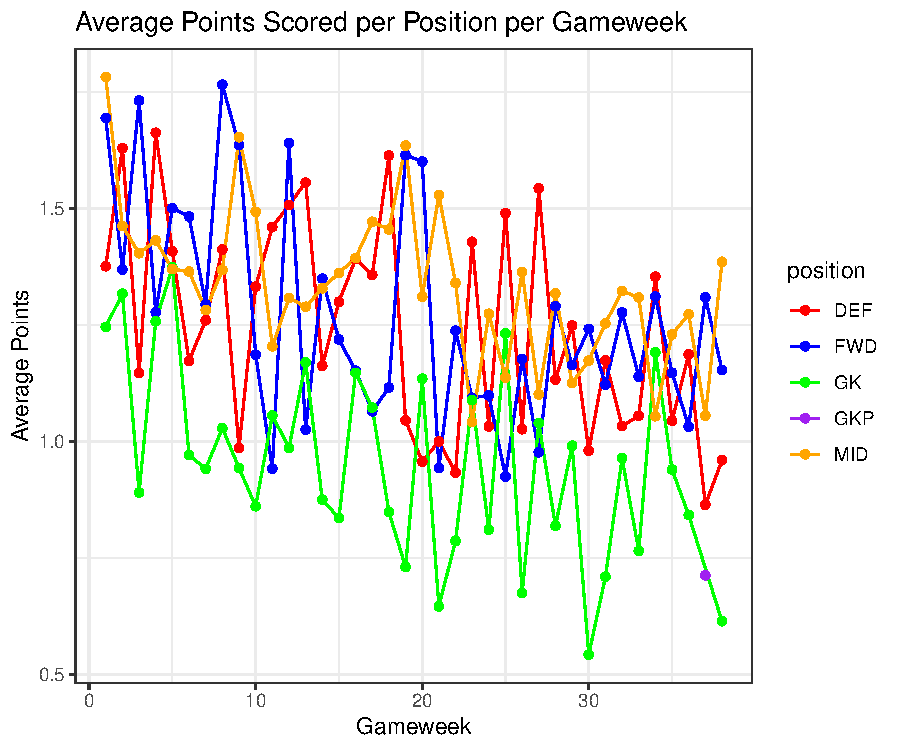
\includegraphics{Fantasy_premier_league_team_prediction_files/figure-latex/unnamed-chunk-4-1} 

}

\caption{Average points per position combined plot\label{Figure3}}\label{fig:unnamed-chunk-4}
\end{figure}

The above figure \ref{Figure3} provides some very valuable information
on how many points are scored per position per game week throughout the
2021/22 premier league season. Each point on the above graph represents
the average points scored for a position (either DEF which represents
defenders, FWD which represents forwards, GK which represents goal
keepers, or MID witch represents midfielders) for that particular game
week. Some important takeaways can be found in this graph.

Goalkeepers on average seem to score the lowest points per game week,
while strikers and defenders seem to have the highest variation and
unpredictability. Midfielders seem to have on average the highest
average points throughout the entire 2021/22 premier league season with
the lowest variation. In order to obtain a clearer picture of the
distribution of points per position the following figure will split the
positions into their own respective plots.

\hypertarget{now-plotting-the-average-points-per-postion-on-differetn-axis-and-plotting-the-overall-average-points-scored-per-postion.}{%
\subsection{Now plotting the average points per postion on differetn
axis and plotting the overall average points scored per
postion.}\label{now-plotting-the-average-points-per-postion-on-differetn-axis-and-plotting-the-overall-average-points-scored-per-postion.}}

\begin{figure}[H]

{\centering \includegraphics{Fantasy_premier_league_team_prediction_files/figure-latex/unnamed-chunk-5-1} 

}

\caption{Average points per postion individual plots\label{Figure4}}\label{fig:unnamed-chunk-5}
\end{figure}

\ref{Figure4} provides a clearer picture of the distribution and
confirms the takeaways made in response to \ref{Figure3}. \ref{Figure4}
places each positions average point distribution throughout the 2021/22
season onto their own plot but with the same axis and places a
horizontal line on the plot that represents the overall average for that
position. It can be confirmed that goal keepers do in fact score on
average the lowest points per game week, defenders and strikers have a
higher variation and midfielders seem to be the best bet to obtain a
higher probability of receiving higher points throughout the season.

The takeaway that can me made from the evidence of \ref{Figure3} and
\ref{Figure4} is that you will want to have as many midfielders in your
team as possible to take advantage of their higher average points and
lower variance.

Next lets look at the most valuable players.

\hypertarget{scatter-plot-for-points-per-value}{%
\subsection{Scatter plot for points per
value:}\label{scatter-plot-for-points-per-value}}

\begin{figure}[H]

{\centering \includegraphics{Fantasy_premier_league_team_prediction_files/figure-latex/unnamed-chunk-6-1} 

}

\caption{Scatter plot of players points per value\label{Figure5}}\label{fig:unnamed-chunk-6}
\end{figure}

The above scatter plot \ref{Figure5} provides us with some more valuable
insight. On the y axis we have the average total points per player and
on the x axis we have the players value. Each point on this scatter plot
provides us with the points per value statistic. In your fantasy premier
league team you will want players with high points per value ratios. In
the plot it is visible that defenders are much cheaper than midfielders
and forwards. Thus, getting some good cheap defenders in your team may
be beneficial.

Furthermore, this plot prints the names of the three players with the
highest points per value ratios. These players are namely, Reece james
(defender), Jack Harrison (midfielder) and Matt Doherty (defender). It
is important to find players that are both cheap and provide good points
to your fantasy team.

Finally, lets evaluate whether having a certain premier league team
dominate your fantasy team is a viable option. This analysis will be
done in the following figure.

\hypertarget{minmean-and-max-points-per-team-for-a-gameweek}{%
\subsection{Min/mean and max points per team for a
gameweek:}\label{minmean-and-max-points-per-team-for-a-gameweek}}

\begin{figure}[H]

{\centering \includegraphics{Fantasy_premier_league_team_prediction_files/figure-latex/unnamed-chunk-7-1} 

}

\caption{Team points min average and max distribution plot\label{Figure6}}\label{fig:unnamed-chunk-7}
\end{figure}

\ref{Figure6} provides insight into the minimum, average and maximum
points scored by premier league players per team in the premier league.
From this figure it can be seen that you would rather want to avoid
having players from Watford, Norwich and Everton due to their low
average points and low maximum points. The teams that you should look to
have players from are Man city, Liverpool and Chelsea. These teams
posses the highest average points and highest total points. Although the
fantasy premier league restriction of a maximum of three players per
team are allowed makes this difficult. This restriction ensures that we
cannot flood our fantasy team with just Man city players or just
Liverpool players. There may however be a case to look to obtain players
from Wolves, Newcastle, Burnley, Southampton and Leicester due to lower
overall range in points, If you are a fantasy premier league player that
values lower risk which is found in lower point variation, these teams
may suit your risk profile.

\hypertarget{conclusions-made-from-data-analysis}{%
\subsection{Conclusions made from data
analysis}\label{conclusions-made-from-data-analysis}}

The important notes made form this data analysis is that, creativity,
ict\_index, influence, threat, selected and transfers in are important
variables to place in the random forests model as they have explanatory
power over the total points variable. Furthermore, when choosing your
formation of your fantasy premier league team you should look to have as
many midfielders as possible and look to obtain players from Man city,
Liverpool or Chelsea.

\hypertarget{machine-learning-model-using-random-forests}{%
\section{Machine learning model using Random
forests}\label{machine-learning-model-using-random-forests}}

The machine learning model that has been selected for predicting the
amount of fantasy points premier league players will score is the random
forests model. The reasoning behind this choice is the ability of a
random forest model to handle large data sets, reduced risk of over
fitting, the results are robust to noise and outliers Breiman
(\protect\hyperlink{ref-breiman2001random}{2001}).

Handling large data sets is important for this project due to the sheer
amount of information available. There are 38 game weeks with over 500
premier league players. Secondly, reduced risk of over fitting is
essential for this project as we are predicting the amount of points
scored by premier league players over different game weeks. Lastly, it
is critical that the model used is robust to outliers since outliers
will be very prevalent in the premier league data sets due to shock
player performances.

This next section will now walk through the setting up process of the
random forests machine learning model.

\hypertarget{setup-process-of-machine-learning-model}{%
\subsection{Setup process of machine learning
model}\label{setup-process-of-machine-learning-model}}

Firstly, before we begin creating the base line random forests model we
need to preprocess the data to ensure the variables are in the correct
format. Upon analyzing the variables in the first section it was found
that the ``value'' variable did not read into R correctly and needs to
be divided by 10. Next a new data set was created that only obtains the
feature variables that will be used, these variables are,
``creativity'', ``ict\_index'', ``influence'', ``selected'', ``threat'',
``transfers\_in'' and also contains the target variable
``total\_points''. These feature variables were chosen through the
analyses done in the data analysis section.

\hypertarget{creating-the-base-random-forests-model}{%
\subsubsection{Creating the base random forests
model}\label{creating-the-base-random-forests-model}}

In this section a base line random forests model will be created, once
created an evaluation of the mean absolute error will be conducted.
Following this, hyper parameter tuning will take place where the model
will be adapted according to the results found from the hyper parameter
tuning. Then the new tuned model will be run and the mean absolute error
will be compared to that of the base line model. The model with the
lowest mean absolute error will be used for the predictions made in the
next section.

In setting up the base line model the 2021/22 premier league data will
be split into a training set and a test set with a 70/30 split. The
model will use repeated cross validation with 5 folds and repeated at
each fold 3 times. Furthermore, the model will use 50 trees. This model
is then run on the 2021/22 data set with the features being, creativity,
ict\_index, influence, threat, selected and transfers in and the target
variable being ``total points''. The model is first trained using the
training data set. The model then using what it has learnt from the
training data set to create predictions on the test data set which it
has not yet seen. Next the mean absolute error will be calculated using
the yardstick method.

\hypertarget{evaluating-the-performance-of-the-base-line-model}{%
\subsubsection{Evaluating the performance of the base line
model}\label{evaluating-the-performance-of-the-base-line-model}}

Using the yardstick method to calculate the mean absolute error of the
base line random forests model the following results are established.
The mean absolute error when using the training data is 0.3231536 and
when using the test data 0.6033058. These results imply that for the
training set, the predicted total points are on average 0.3231536 points
off the true total points value and 0.6033058 points off when the test
data set is used.

\begin{verbatim}
## [1] 0.3231536
\end{verbatim}

\begin{verbatim}
## [1] 0.6033058
\end{verbatim}

Now hyper parameter tuning on the amount of folds in the cross
validation, the value for mtry and the amount of trees will be
conducted. Once conducted the new model will be run and the mean
absolute error will be evaluated.

\hypertarget{hyper-parameter-tuning}{%
\subsection{Hyper parameter tuning}\label{hyper-parameter-tuning}}

\hypertarget{mtry-hyper-parameter-tuning}{%
\subsubsection{mtry hyper parameter
tuning}\label{mtry-hyper-parameter-tuning}}

Firstly, we will be tuning the mtry hyper parameter of the model. The
tuning grid consists of (1, 2, 3, 4, 5). In the process of tuning this
parameter the model will run 5 different times changing just the mtry
value from 1 through 5. The model will then pick the mtry value which is
associated with the lowest mean absolute error.

After completing the tuning process the mtry value of 2 is associated
with the lowest mean absolute error. This mtry value is the same as the
one used in the base line model and thus we do not need to change this
parameter value.

\hypertarget{k-fold-hyper-parameter-tuning}{%
\subsubsection{k-fold Hyper parameter
tuning}\label{k-fold-hyper-parameter-tuning}}

Secondly, evaluating how many folds to be used in the cross validation
process will be calculated. A fold range of (5, 10, 15, 20) will be
evaluated. Thus, again the model will be run 4 different times with
differing k-fold values in an attempt to find the most appropriate k
value that results in the lowest mean absolute error.

After running through the range of k-fold values a k value of 5 is found
to be the most optimal.Like that of the mtry parameter value, this is
the same k-fold value that was used in the baseline model and thus, the
base line model is yet to be adapted.

\hypertarget{ntree-hyper-parameter-tuning}{%
\subsubsection{ntree hyper parameter
tuning}\label{ntree-hyper-parameter-tuning}}

The last parameter value to be tuned is the amount of trees used in the
random forests model. A tuning grid of (50, 100, 150) will be used. The
model will run 3 times iterating through the different tree values and
will look for the tree parameter that is associated with the lowest mean
absolute error.

After running through the tuning grid of differing tree values, a tree
value of 150 is found to create the lowest mean absolute error. This
value of ntree = 150 differs from the base line model which used a ntree
value of 50. Thus, the base line model needs to be adapted.

\hypertarget{best-model-after-hyper-parameter-tuning}{%
\subsection{Best model after hyper parameter
tuning}\label{best-model-after-hyper-parameter-tuning}}

After conducting some hyper parameter tuning on the parameter of mtry,
k-fold and ntree, the new tuned model is created. This model still
splits the 2021/22 data into a training set ad a test set with a 70/30
split. This new random forests model uses repeated cross validation with
5 folds and is repeated three times at each fold and uses 150 trees. The
model is trained using the training set and creates predictions on the
test set which it has not yet seen. Once again the features are,
creativity, ict\_index, influence, threat, selected and transfers in and
the target variable being ``total points''.

After this model is run, the mean absolute error will be calculated and
compared to that of the baseline model.

\hypertarget{evaluating-the-performance-of-the-tuned-model}{%
\subsection{Evaluating the performance of the tuned
model}\label{evaluating-the-performance-of-the-tuned-model}}

Using the yardstick method to obtain the mean absolute error of the
tuned model we get the following results of 0.3210782 when the training
data is used and 0.6019206 when the test data set is used. This means
that on average when using the training data set the predicted total
points value is off by 0.3210782 points and when using the test set the
predicted values are off by 0.6019206 points.

When comparing these mean absolute error values to that of the once
obtained in the base line model, the tuned model performs slightly
better. With respect to the training data predictions the tuned model
performs on average better than the base line model by 0.0020754 points
and with respect to the predictions made on the test data, the tuned
model performs on average better than the base line model by 0.0013852
points. Thus by increasing the amount of trees from 50 to 150 the model
only improves slightly. This provides evidence that although increasing
the amount of trees further than 150 may decrease the error it will not
be worth the additional computational time.

Thus the tuned model will be used for the predictions that will be made
in the following sections.

\begin{verbatim}
## [1] 0.3210782
\end{verbatim}

\begin{verbatim}
## [1] 0.6019206
\end{verbatim}

\hypertarget{the-important-restrictions-to-note-when-building-your-fantasy-premier-league-team}{%
\section{The important restrictions to note when building your fantasy
premier league
team}\label{the-important-restrictions-to-note-when-building-your-fantasy-premier-league-team}}

There are three important restrictions that need to be taken into
account when building your fantasy premier league team. The first being
that your are only allowed a maximum of three players per premier league
team in your fantasy premier league team. Secondly, your total team cost
cannot exceed 100 mil. Lastly, you need to pick which formation you want
to play. This means that you have to have at least one goal keeper,
between 3-5 defenders, between 3-5 midfielders, and between 1-3
forwards. Due to the analyses made in the data analysis section I will
be choosing a formation that has as many midfielders as possible and
seeing that you can get cheap defenders that can score lots of points I
will be going for more defenders than strikers to keep the cost down.
Thus the formation chosen for this project is 1 defender, 3 defenders, 5
midfielders and 2 strikers.

\hypertarget{time-for-predictions}{%
\section{Time for predictions}\label{time-for-predictions}}

\hypertarget{predictions-on-the-202223-data-set}{%
\subsection{Predictions on the 2022/23 data
set}\label{predictions-on-the-202223-data-set}}

The new tuned random forests model is used to create predictions on the
2022/23 data set. Firstly, the 2022/23 data set must be cleaned to
ensure that the 2022/22 and 2022/23 data sets contain the same
variables. Once this was done, the predictions on the 2022/23 data set
could commence.

Once predictions were made, this prediction variable is added back to
the main data set so that we could extract variables such as the name of
the player the actual points scored, the predicted points scored, what
team they play for, which potion they play in and their value.

\hypertarget{game-week-predictions}{%
\subsection{Game week predictions}\label{game-week-predictions}}

\hypertarget{beggining-of-the-season-predtions}{%
\subsubsection{Beggining of the season
predtions}\label{beggining-of-the-season-predtions}}

\hypertarget{game-week-9-predictions-and-actual-best-team}{%
\paragraph{Game week 9 predictions and actual best
team}\label{game-week-9-predictions-and-actual-best-team}}

The following 11 players are apart of the predicted fantasy team for
game week 9:

\begin{verbatim}
## # A tibble: 11 x 6
##    names_22_23              predicted_points total_points position team    value
##    <chr>                               <dbl>        <dbl> <chr>    <chr>   <dbl>
##  1 Erling Haaland                      19.4            23 FWD      Man Ci~  12.1
##  2 Phil Foden                          16.3            19 MID      Man Ci~   8  
##  3 Leandro Trossard                    16.0            20 MID      Bright~   6.6
##  4 James Maddison                      15.3            18 MID      Leices~   8  
##  5 Roberto Firmino                     13.9            12 FWD      Liverp~   7.9
##  6 Miguel Almirón Rejala               13.9            15 MID      Newcas~   5  
##  7 Jarrod Bowen                        10.6            14 MID      West H~   8.1
##  8 Conor Coady                          9.12            9 DEF      Everton   4.8
##  9 Thiago Emiliano da Silva             7.71            6 DEF      Chelsea   5.4
## 10 Vitalii Mykolenko                    6.16            2 DEF      Everton   4.5
## 11 Illan Meslier                        4.89           11 GK       Leeds     4.5
\end{verbatim}

The following 11 players are apart of the actual best team for game week
9:

\begin{verbatim}
## # A tibble: 11 x 6
##    names_22_23           predicted_points total_points position team      value
##    <chr>                            <dbl>        <dbl> <chr>    <chr>     <dbl>
##  1 Erling Haaland                   19.4            23 FWD      Man City   12.1
##  2 Leandro Trossard                 16.0            20 MID      Brighton    6.6
##  3 Phil Foden                       16.3            19 MID      Man City    8  
##  4 James Maddison                   15.3            18 MID      Leicester   8  
##  5 Miguel Almirón Rejala            13.9            15 MID      Newcastle   5  
##  6 Jarrod Bowen                     10.6            14 MID      West Ham    8.1
##  7 Roberto Firmino                  13.9            12 FWD      Liverpool   7.9
##  8 Illan Meslier                     4.89           11 GK       Leeds       4.5
##  9 Thilo Kehrer                      2.73           10 DEF      West Ham    4.5
## 10 Conor Coady                       9.12            9 DEF      Everton     4.8
## 11 Timothy Castagne                  2.27            8 DEF      Leicester   4.4
\end{verbatim}

In game week 9 the prediction model correctly predicted 9 out of the 11
players with a total of 149 points out of a maximum of 159 points
obtained by the actual best team.

\hypertarget{middle-of-the-season-predictions}{%
\subsubsection{Middle of the season
predictions}\label{middle-of-the-season-predictions}}

\hypertarget{game-week-16-predictions-and-actual-best-team}{%
\paragraph{Game week 16 predictions and actual best
team}\label{game-week-16-predictions-and-actual-best-team}}

The following 11 players are apart of the predicted fantasy team for
game week 16:

\begin{verbatim}
## # A tibble: 11 x 6
##    names_22_23           predicted_points total_points position team      value
##    <chr>                            <dbl>        <dbl> <chr>    <chr>     <dbl>
##  1 Ivan Toney                       15.7            13 FWD      Brentford   7.4
##  2 Rodrigo Moreno                   13.9            13 MID      Leeds       6.3
##  3 Darwin Núñez Ribeiro             13.6            13 FWD      Liverpool   9  
##  4 Martin Ødegaard                  13.0            16 MID      Arsenal     6.4
##  5 Rodrigo Bentancur                12.5            14 MID      Spurs       5.4
##  6 Crysencio Summerville             9.50            7 MID      Leeds       4.4
##  7 Phil Foden                        9.42            9 MID      Man City    8.3
##  8 Andrew Robertson                  9.02            9 DEF      Liverpool   6.7
##  9 Ben Davies                        8.96            7 DEF      Spurs       4.9
## 10 Mathias Jorgensen                 5.36            2 DEF      Brentford   4  
## 11 Danny Ward                        5.00           11 GK       Leicester   4.1
\end{verbatim}

The following 11 players are apart of the actual best team for game week
16:

\begin{verbatim}
## # A tibble: 11 x 6
##    names_22_23          predicted_points total_points position team      value
##    <chr>                           <dbl>        <dbl> <chr>    <chr>     <dbl>
##  1 Martin Ødegaard                13.0             16 MID      Arsenal     6.4
##  2 Rodrigo Bentancur              12.5             14 MID      Spurs       5.4
##  3 Christian Eriksen               0.304           13 MID      Man Utd     6.3
##  4 Rodrigo Moreno                 13.9             13 MID      Leeds       6.3
##  5 Ivan Toney                     15.7             13 FWD      Brentford   7.4
##  6 Darwin Núñez Ribeiro           13.6             13 FWD      Liverpool   9  
##  7 Joe Willock                     9.12            11 MID      Newcastle   4.9
##  8 Danny Ward                      5.00            11 GK       Leicester   4.1
##  9 Andrew Robertson                9.02             9 DEF      Liverpool   6.7
## 10 Benjamin White                  3.11             8 DEF      Arsenal     4.6
## 11 Fabian Schär                    4.22             7 DEF      Newcastle   4.9
\end{verbatim}

In game week 16 the prediction model correctly predicted 7 out of the 11
players with a total of 114 points out of a maximum of 128 points
obtained by the actual best team.

\hypertarget{end-of-the-season-predictions}{%
\subsubsection{End of the season
predictions}\label{end-of-the-season-predictions}}

\hypertarget{game-week-35-predictions-and-actual-best-team}{%
\paragraph{Game week 35 predictions and actual best
team}\label{game-week-35-predictions-and-actual-best-team}}

The following 11 players are apart of the predicted fantasy team for
game week 35:

\begin{verbatim}
## # A tibble: 11 x 6
##    names_22_23                predicted_points total_points position team  value
##    <chr>                                 <dbl>        <dbl> <chr>    <chr> <dbl>
##  1 Dwight McNeil                         17.1            21 MID      Ever~   5.1
##  2 Ilkay Gündogan                        13.9            13 MID      Man ~   7.3
##  3 James Ward-Prowse                     13.4            13 MID      Sout~   6.1
##  4 Abdoulaye Doucouré                    13.3            13 MID      Ever~   5.3
##  5 James Maddison                        12.9             9 MID      Leic~   7.9
##  6 Toti António Gomes                     9.64           14 DEF      Wolv~   3.8
##  7 Harry Kane                             9.13            8 FWD      Spurs  11.4
##  8 Lyanco Silveira Neves Voj~             7.78            6 DEF      Sout~   4.4
##  9 Benoît Badiashile                      7.71            7 DEF      Chel~   5  
## 10 João Félix Sequeira                    5.84            7 FWD      Chel~   7.2
## 11 Nick Pope                              4.96            2 GK       Newc~   5.4
\end{verbatim}

The following 11 players are apart of the actual best team for game week
35:

\begin{verbatim}
## # A tibble: 11 x 6
##    names_22_23         predicted_points total_points position team        value
##    <chr>                          <dbl>        <dbl> <chr>    <chr>       <dbl>
##  1 Dwight McNeil                  17.1            21 MID      Everton       5.1
##  2 Toti António Gomes              9.64           14 DEF      Wolves        3.8
##  3 Abdoulaye Doucouré             13.3            13 MID      Everton       5.3
##  4 Ilkay Gündogan                 13.9            13 MID      Man City      7.3
##  5 James Ward-Prowse              13.4            13 MID      Southampton   6.1
##  6 Pedro Porro                     6.08           12 DEF      Spurs         4.8
##  7 Saïd Benrahma                   9.86           11 MID      West Ham      5.5
##  8 Virgil van Dijk                 6.99           11 DEF      Liverpool     6.6
##  9 Aaron Ramsdale                  3.55           10 GK       Arsenal       4.8
## 10 Harry Kane                      9.13            8 FWD      Spurs        11.4
## 11 João Félix Sequeira             5.84            7 FWD      Chelsea       7.2
\end{verbatim}

In game week 35 the prediction model correctly predicted 7 out of the 11
players with a total of 113 points out of a maximum of 133 points
obtained by the actual best team.

\hypertarget{conclusion}{%
\section{Conclusion}\label{conclusion}}

TO conclude, by using the above fantasy premier league prediction model
I was able to predict up to 9 out of the 11 players that would make the
best team of the week with on average 6/7 players correctly predicted.
However, this model can be adapted if it were to actually be used for
selecting a fantasy team throughout the season. This is because what
this model can do is predict a brand new team each game week fairly
well, which is not allowed in the actual fantasy game, since you can
only make a few substitutions per week.

\newpage

\hypertarget{references}{%
\section*{References}\label{references}}
\addcontentsline{toc}{section}{References}

\hypertarget{refs}{}
\begin{CSLReferences}{1}{0}
\leavevmode\vadjust pre{\hypertarget{ref-breiman2001random}{}}%
Breiman, L. 2001. Random forests. \emph{Machine learning}. 45:5--32.

\end{CSLReferences}

\hypertarget{appendix}{%
\section*{Appendix}\label{appendix}}
\addcontentsline{toc}{section}{Appendix}

\hypertarget{appendix-a}{%
\subsection*{Appendix A}\label{appendix-a}}
\addcontentsline{toc}{subsection}{Appendix A}

Some appendix information here

\hypertarget{appendix-b}{%
\subsection*{Appendix B}\label{appendix-b}}
\addcontentsline{toc}{subsection}{Appendix B}

\bibliography{Tex/ref}





\end{document}
